% Presentation: Introduction to MOM
%     Location: CoE CMS Winter School, 12 July 2012
%       Author: Marshall Ward
%-----------------------------------------------------------------------------%
\documentclass[red]{beamer}

% Font configuration
\usepackage{pxfonts}

% Packages
\usepackage{listings}
\usepackage{hyperref}
\usepackage[squaren]{SIunits}

\usepackage{color}
\definecolor{ltblue}{rgb}{0.9, 0.9, 1.0}
\definecolor{dkgreen}{rgb}{0,0.6,0}
\definecolor{gray}{rgb}{0.5,0.5,0.5}
\definecolor{mauve}{rgb}{0.58,0,0.82}

% Beamer configuration
\usetheme{Frankfurt}

% LaTeX configuration
\graphicspath{{figures/}}

%=============================================================================%
\title{An Introduction to MOM}
\date{12 July 2012}

%=============================================================================%
\begin{document}
% Listings settings
\lstset{
    language=bash,
    basicstyle=\ttfamily,
    showspaces=false,
    showstringspaces=false,
    backgroundcolor=\color{ltblue},
    numberstyle=\tiny\color{gray},
    keywordstyle=\color{blue},
    commentstyle=\color{dkgreen},
    stringstyle=\color{mauve}
}

%-----------------------------------------------------------------------------%
\begin{frame}
    \titlepage
\end{frame}

%=============================================================================%
\section[Overview]{MOM4 Overview}

%-----------------------------------------------------------------------------%
\begin{frame}
    \frametitle{MOM4 Dynamic Core}
    
    \begin{itemize}
        \item Hydrostatic, Boussinesq
        \item Orthogonal Horizontal Grids
        \item Generalised vertical grids: $z, p$
		\item Explicit free surface
		\item Modern thermodynamic support
        \item Partial grid topograpy
    \end{itemize}
\end{frame}    

%-----------------------------------------------------------------------------%
\begin{frame}
    \frametitle{Orthogonal Horizontal Grids}
    
    \begin{center}
        \includegraphics<1>[width=0.7\textwidth]{merc_tripolar.pdf}
        \includegraphics<2>[width=0.5\textwidth]{nh_tripolar.pdf}
        \includegraphics<2>[width=0.5\textwidth]{sh_tripolar.pdf}
        \includegraphics<3>[width=0.7\textwidth]{merc_auscom.pdf}
    \end{center}
\end{frame}

%-----------------------------------------------------------------------------%
\begin{frame}
    \frametitle{Generalised Vertical Grids}
    
    \begin{itemize}
        \item Depth coordinates $z$ (Boussinesq)
         
        \item Hydrostatic pressure coordinates $p$ (Non-Boussinesq)
        
        \item Quasi-horizontal vertical grids:
            $z^* = H(\mathbf{x}) \left(\frac{z - \eta}{H + \eta}\right)$
        
        \item Limited support for terrain-following ($\sigma$) coordinates
    \end{itemize}
\end{frame}

%-----------------------------------------------------------------------------%
\begin{frame}
    \frametitle{Quasi-horizontal Vertical Grids}
    
    \begin{center}
        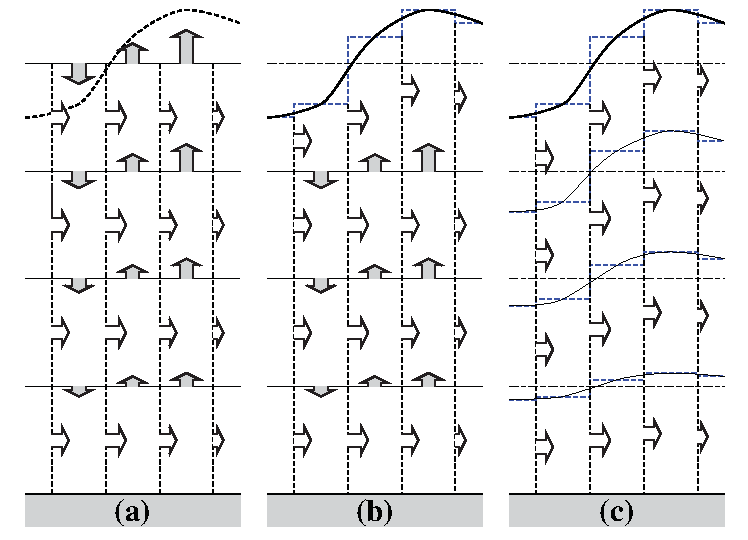
\includegraphics[width=0.8\textwidth]{zstar.pdf}
    \end{center}
    
    {\tiny "NEMO Ocean Engine", Madec et al. (2012)}
\end{frame}

%-----------------------------------------------------------------------------%
\begin{frame}
    \frametitle{Alternative Ocean Models}
    
    \begin{itemize}
        \item MITgcm: finite-volume, nonhydrostatic
        \item GOLD: isopycnal
        \item ROMS: "regional", sigma-coordinate
        \item HYCOM: "hybrid" vertical grid ($z$-$\rho$-$\sigma$)
    \end{itemize}
    
    "MOM-like" (Bryan-Cox) Ocean Models
    \begin{itemize}
        \item NEMO: C-grid
        \item POP2 (part of CESM)
        \item COCO (part of MIROC)
    \end{itemize}
\end{frame}

%=============================================================================%
\section{MOM4 Quick User's guide}
%-----------------------------------------------------------------------------%
\begin{frame}
    \frametitle{Constructing a MOM4 Experiment}
    
    \begin{itemize}
        \item Acquiring the source code
        \item Creating a model grid
        \item Model configuration
        \item Compiling and running the model
    \end{itemize}

\end{frame}

%-----------------------------------------------------------------------------%
\begin{frame}[fragile]
    \frametitle{Acquiring the source code}
    
    Up-to-date versions of the source code are available on a subversion (svn)
    server hosted by NCI:
    
    \begin{lstlisting}
# Enter as one line
svn co https://access-svn.nci.org.au/mom4
               /branches/local_changes
    \end{lstlisting}
    Contact NCI for access (IP address required)
    
    \begin{itemize}
        \item \lstinline|mom4/trunk|: GFDL code release mirror
        \item \lstinline|local_changes|: Stable release on vayu
        \item \lstinline|future_local_changes|: Experimental release on vayu
    \end{itemize}
    
    \textit{Note: Expect changes to this in the future}
\end{frame}

%-----------------------------------------------------------------------------%
\begin{frame}
    \frametitle{Creating a model grid}
    
    Mosaic grid generation for ocean-only (\textit{solo}) simulations:
    \begin{itemize}
        \item Vertical grid
        \item Horizontal grid
        \item Mosaic manifest file
        \item Topography
    \end{itemize}
    
    Caveats:
    \begin{itemize}
        \item "Supergrid" output: $N$ cells, $2N+1$ grid points
        \item New toolset, differs from previous grid format
        \item Mosaic is mostly finished, but still under development
    \end{itemize}
\end{frame}

%-----------------------------------------------------------------------------%
\begin{frame}[fragile]
    \frametitle{Vertical Grid Generation}
    
    Uniform vertical grid:
    \begin{lstlisting}
# From the source directory
> cd src/tools/ocean_vgrid
> make
> ./ocean_vgrid \
     --nbnds 3 \
     --bnds 0,4000 \
     --nz 40
    \end{lstlisting}
    
    Variable resolution:
    \begin{lstlisting}
> ./ocean_vgrid \
     --nbnds 4
     --bnds 0,100,500,4000
     --nz 10,10,20
    \end{lstlisting}
\end{frame}
%-----------------------------------------------------------------------------%
\begin{frame}[fragile]
    \frametitle{Horizontal Grid Generation}
   
    Uniform $1^\circ$ spherical grid:
    \begin{lstlisting}
> cd src/tools/make_hgrid
> make
> ./make_hgrid \
     --grid_type regular_lonlat_grid \
     --nxbnd 2 \
     --nybnd 2 \
     --xbnd 0,40 \
     --ybnd -80,80 \
     --nlon 40 \
     --nlat 160
    \end{lstlisting}
\end{frame}

%-----------------------------------------------------------------------------%
\begin{frame}[fragile]
    \frametitle{Mosaic manifest file}
    
    \textit{Mosaic} files contain metadata to grid files:
    \begin{lstlisting}
> cd src/tools/make_solo_mosaic
> make
> ./make_solo_mosaic \
     --num_tiles 1 \
     --dir . \
     --periodx 40
    \end{lstlisting}
\end{frame}

%-----------------------------------------------------------------------------%
\begin{frame}[fragile]
    \frametitle{Topography generation}
   
    Idealised flat-bottom topography
    \begin{lstlisting}
> cd src/tools/make_topog
> make
> ./make_topog \
     --mosaic solo_mosaic.nc \
     --topog_type rectangular_basin \
     --basin_depth 4000
    \end{lstlisting}

    Note: For the parallel MPI version, use
    \begin{lstlisting}
> make -f Makefile_mpi
    \end{lstlisting}
\end{frame}

%-----------------------------------------------------------------------------%
\begin{frame}
    \frametitle{Interpolated Topography}

    Interpolated from observations:
    \lstinputlisting{scripts/interp_topog.sh}

\end{frame}
%-----------------------------------------------------------------------------%
\begin{frame}
    \frametitle{Model Configuration}
    
    Main configuration files:
    \begin{itemize}
        \item \lstinline|input.nml|: Most configuration settings (Fortran
            namelist)
        \item \lstinline|diag_table|: Diagnostic output
        \item \lstinline|data_table|: Input fields and boundary conditions
        \item \lstinline|field_table|: Initial conditions, advection
            configuration
    \end{itemize}
\end{frame}

%=============================================================================%
\end{document}
